\section{Cargas de diseño}
Los cálculos y las consideraciones propias para el análisis con cargas de gravedad y de sismo, así como el diseño estructural del edificio se realizarán de acuerdo a lo especificado en las normas NTE E-020 Metrado de Cargas, NTE E-030 Diseño Sismorresistente, NTE E-060 Diseño de Concreto Armado.

\subsection{Cargas Muertas}

Las cargas muertas se determinan del cálculo directo del peso de todos los componentes estructurales y de elementos no estructurales cuya posición no se modificará durante la vida útil de la edificación. La norma E-020 del RNE nos proporciona algunos pesos unitarios para calcular la carga muerta, en nuestro caso tenemos:
\vspace{0.8cm}
% Table generated by Excel2LaTeX from sheet 'Hoja1'
\begin{table}[htbp]
  \centering
 % \caption{Add caption}
    \begin{tabular}{lrl}
    Concreto armado & :     & 2400 kg/m\raisebox{1ex}{\scriptsize{3}}\\
              &       &  \\
    Muro de albañilería hueca & :     & 1350 kg/m\raisebox{1ex}{\scriptsize{3}} \\
              &       &  \\
    Muro de albañilería solida                              & :     & 1800 kg/m\raisebox{1ex}{\scriptsize{3}}  \\
              &       &  \\
    Mortero de cemento & :     & 2000 kg/m\raisebox{1ex}{\scriptsize{3}}  \\
              &       &  \\
    Piso terminado (pt)  & :     & 100 kg/m\raisebox{1ex}{\scriptsize{2}}  \\
    \end{tabular}%
  \label{tab:addlabel}%
\end{table}%

La carga muerta lo calcula el programa, pero adicionalmente se consideró una sobrecarga permanente de 100 kg/m\raisebox{1ex}{\scriptsize{2}} que incluye piso terminado.
También se incluyó las cargas distribuidas directamente sobre vigas debido a las tabiquerías de espesor 15 cm. Los muros se suponen construidos con ladrillos pandereta cuyo peso especifico se extrae de la norma E-020:

\begin{figure}[h!]
    \centering
    \caption{Peso unitario de tabiquería}
    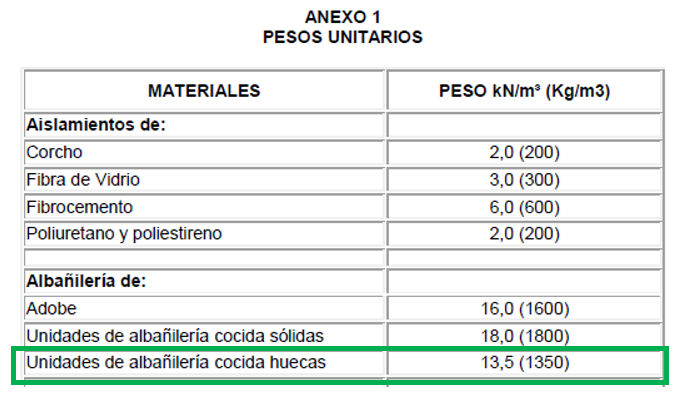
\includegraphics[scale=0.7]{IMAGENES/3.PNG}
    \caption*{\small Fuente: \it \cite{E-020}}
    \label{fig:my_label}
\end{figure}

\newpage

\subsection{Cargas Vivas}
La carga de piso que se va aplicar a un área determinada de una edificación depende de su pretendida utilización u ocupación. Estas cargas se deben a los seres humanos, al equipo, al almacenamiento en general, a los automóviles, etc., debido a que estas cargas son de naturaleza aleatoria, no hay una forma precisa para aplicar las cargas reales a un área dada. Por esa razón se especifican como cargas distribuidas uniformemente en el área. Cabe indicar que estas cargas son extremamente conservadoras debido a la incertidumbre acerca de cómo pudieran distribuirse las cargas reales. La norma E020 nos da cargas distribuidas para distintos tipos de ocupación o uso, en nuestro caso para una edificacion de vivienda se tiene:  

\begin{figure}[h]
    \centering
    \caption{Carga viva para viviendas}
    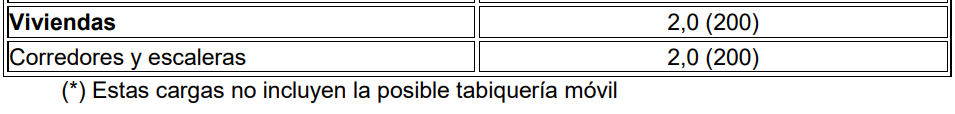
\includegraphics[scale=0.8]{IMAGENES/4.PNG}
    \label{fig:my_label}
    \caption*{\small Fuente: \it \cite{E-020}}
\end{figure}

\begin{figure}[h]
    \centering
    \caption{Carga viva en azoteas}
    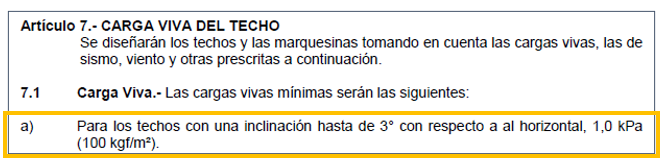
\includegraphics[scale=1]{IMAGENES/7.PNG}
    %\label{fig:my_label}
    \caption*{\small Fuente: \it \cite{E-020}}
\end{figure}

\newpage